% !TEX root = ../../../main.tex
% 来源：中学数学实验教材·第三册（高中数学）
% 章节：任意角的三角函数 / 弧和角的概念及其度量
% 原始文件：6.tex，行 373-401
% 类型：tikz
% ---
\begin{tikzpicture}[>=latex]
\begin{scope}
    \draw[->](-2,0)--(2,0)node[right]{$x$};
    \draw[->](0,-2)--(0,2)node[right]{$y$};
\draw (0,0)--(30:2.5)node[right]{$B$};
\draw[->] (.75,0) arc (0:30:.75);
\draw[->] (1,0) arc (0:-330:1);
\node at (.2,-.2){$O$};
\node at (15:1){$\tfrac{\pi}{6}$};
\node at (2,.5){$\tfrac{13\pi}{6}$};
\node at (.5,1.2){$-\tfrac{11\pi}{6}$};
\draw(1.5,0) arc (0:270:1.5);
\draw [->] (0,-1.5) arc (270:384:1.7);
\node at (0,-2.5){(1)};
\end{scope}
\begin{scope}[xshift=6cm]
    \draw[->](-2,0)--(2,0)node[right]{$x$};
    \draw[->](0,-2)--(0,2)node[right]{$y$};
    \draw (0,0)--(-60:2.5)node[right]{$B$};
    \draw[->] (.75,0) arc (0:-60:.75);
    \draw[->] (1,0) arc (0:300:1);
    \node at (.2,.2){$O$};
    \node at (-30:1){$-\tfrac{\pi}{3}$};
    
\node at (1,1){$\tfrac{5\pi}{3}$};
\node at (0,-2.5){(2)};

\end{scope}
\end{tikzpicture}   
